%%%%%%%%%%%%%%%%%%%%%%%%%%%%%%%%%%%%%%%%%%%%%%%%%%%%%%%%%%%%%%%%%%%%
% This is a thesis template for Gebze Technical University.
%
% Please only edit the areas proceeded by a comment starting with %%
% otherwise the template may be broken.
%
% This file is only to be used for editing the general fields
% and inputting the body of the thesis in the designated areas.
% Please write the body of the thesis in separate files, and input
% them as shown in the comment preceding the area.
%
% Created in Aug 2021 by Usama Derbashi.
%%%%%%%%%%%%%%%%%%%%%%%%%%%%%%%%%%%%%%%%%%%%%%%%%%%%%%%%%%%%%%%%%%%%
\documentclass[12pt]{report}


% Language and typeset setting
\usepackage[english]{babel}
\usepackage[a4paper,top=25mm,bottom=25mm,left=40mm,right=25mm]{geometry}
\usepackage[onehalfspacing]{setspace}
\usepackage{algorithm, algpseudocode}
\usepackage{indentfirst}
\setlength{\parindent}{1cm}
\setlength{\abovecaptionskip}{12pt plus 0pt minus 0pt}
\setlength{\belowcaptionskip}{12pt plus 0pt minus 0pt}
\setlength{\textfloatsep}{18.0pt plus 0.0pt minus 0.0pt}
\setlength{\floatsep}{18.0pt plus 0.0pt minus 0.0pt}
\setlength{\intextsep}{18.0pt plus 0.0pt minus 0.0pt}
\setlength{\skip\footins}{18.0pt plus 0.0pt minus 0.0pt}

% Core packages and settings
\usepackage[colorlinks=false]{hyperref}
\usepackage{amsmath}

\usepackage{titlesec} %setting the titles of chapters and sections
\setcounter{secnumdepth}{4}
\setcounter{tocdepth}{4}
\titleformat{\chapter}[hang]{\normalfont\bfseries\MakeUppercase}{}{0pt}{\LARGE\thechapter. }
\titleformat{\section}[hang]{\normalfont\bfseries}{}{0pt}{\Large\thesection. }
\titleformat{\subsection}[hang]{\normalfont\bfseries}{}{0pt}{\large\thesubsection. }
\titleformat{\subsubsection}[hang]{\normalfont\bfseries}{}{0pt}{\large\thesubsubsection. }
\titlespacing*{\chapter}{0pt}{0pt}{18pt}
\titlespacing*{\section}{0pt}{18pt}{18pt}
\titlespacing*{\subsection}{0pt}{18pt}{18pt}
\titlespacing*{\subsubsection}{0pt}{18pt}{18pt}

\usepackage{graphicx}
\graphicspath{{./Imgs/}} %pointing the directory of images

\usepackage{fancyhdr} % setting footers
\usepackage{etoolbox} 
\renewcommand{\headrulewidth}{0pt}
\patchcmd{\chapter}{\thispagestyle{plain}}{\thispagestyle{fancy}}{}{}
\pagestyle{fancy}
\fancyhf{}
\fancyfoot[C]{\fontsize{11pt}{11pt}\thepage}

\usepackage[style=ieee]{biblatex}
\addbibresource{refs.bib}
\usepackage{csquotes}% Needed for babel(in biblatex)

\usepackage[bottom, perpage]{footmisc}%% amkes footnotes at the bottom

\usepackage{GTUThesis}


% Additional packages if needed
%% For the sake of not messing the template add them here
\usepackage{lipsum}


% Important information
%% Make sure to enter all the info below
\title{Smart Minibar}
\author{Muhammed Alperen Karaçete}
\faculty{Faculty of Engineering}
\department{Computer Engineering Department}
\supervisor{Dr. Mehmet GÖKTÜRK}
\theyear{2023}


\begin{document}

%Front Matter
\pagenumbering{roman} %start with roman numbering 
\projecttitlepageenglish
\maketitle
\setcounter{page}{3} %the first two title pages are not counted so this is a buffer
\begin{outertitles} % makes titles centred

%% below enter as follows 
%% {DATE_OF_DEMO}{JURY}
%% Note that JURY should be comma separated
\makejury{}{}
\chapter*{Abstract}
\addcontentsline{toc}{chapter}{Abstract}

%% Edit below this line
The Smart Minibar with Object Detection using Webcam and Firebase is an innovative system that combines a webcam, the MobileNet SSD v2 object detection model, and Firebase as the real-time database. The purpose of this project is to create a smart minibar that can track and manage the inventory of items inside it, provide real-time monitoring, and automate the billing process based on the items taken by the user.

The system utilizes a webcam connected to the minibar, which captures real-time images of the minibar's contents. These images are then processed using the MobileNet SSD v2 model, a trained object detection model capable of recognizing and localizing various objects within the minibar. To train the model, a set of training images consisting of labeled examples of minibar items is used. This enables the model to accurately detect and classify the items.Used products in this project are Cola,Fanta,Sprite and water.

Firebase serves as the real-time database for storing and managing the inventory details of the minibar items. The database stores information such as item names, quantities, and user informations. The system records the user's actions, tracks the items taken from the minibar, and updates the inventory and user's bill in the Firebase database accordingly.
%% Until here
\vfill
%% Edit after {Keywords:}
\clearpage
\chapter*{Özet}
\addcontentsline{toc}{chapter}{Özet}

%% Edit below this line
Akıllı Minibar, bir webcam, MobileNet SSD v2 nesne algılama modeli ve Firebase'in gerçek zamanlı veritabanını bir araya getiren yenilikçi bir sistemdir. Bu proje,minibar içindeki ürünlerin miktarını takip etmek ve yönetmek, gerçek zamanlı izleme sağlamak ve kullanıcı tarafından alınan ürünlere dayalı olarak fatura sürecini otomatikleştirmek amacıyla akıllı bir minibar oluşturmayı amaçlamaktadır.

Sistem, minibara bağlı olan bir webcam'i kullanır ve minibarın içeriğinin gerçek zamanlı görüntülerini inceler. Bu görüntüler daha sonra MobileNet SSD v2 modeli kullanılarak eğitilir. Eğitilmiş nesne algılama modeli, minibar içindeki çeşitli nesneleri tanımlayabilen ve sayabilen bir yeteneğe sahiptir. Modelin eğitimi için, minibar ürünlerinin etiketlenmiş örneklerinden oluşan bir eğitim görüntü seti kullanılır. Bu, modelin ürünleri doğru bir şekilde algılayıp sınıflandırabilmesini sağlar.Bu projede kullanılan ürünler ise Cola,Fanta,Sprite ve sudur.

Firebase, minibar ürünlerinin envanter detaylarını depolamak ve yönetmek için gerçek zamanlı bir veritabanı olarak görev yapar. Veritabanı, ürün adları ve miktarları ve kullanıcı bilgilerini saklar. Sistem, kullanıcının eylemlerini kaydeder, minibardan alınan ürünleri takip eder ve envanteri ve kullanıcının faturasını Firebase veritabanında günceller.

%% Until here
\vfill
%% Edit after {Anahtar Kelimeler:}
\clearpage
\input{./Body/Frontmatter/Acknowledgement}
\chapter*{List of Symbols and Abbreviations}
\addcontentsline{toc}{chapter}{List of Symbols and Abbreviations}

\begin{tabular}{lcl}
    \textbf{Symbol or}&&\\
    \textbf{Abbreviation} &:& \textbf{Explanation}\\
    
    %% Edit below in the format
    %% XYZ &:& EXPLANATION\\
    %% where XYZ is the acronym or symbol
    %% and EXPLANATION is the explanation of it
    %% make sure not to forget &:& between them, and \\ at the end of EXPLANATION
    
    
    
    %% Until here
\end{tabular}

\clearpage

\tableofcontents
\addcontentsline{toc}{chapter}{Contents}
\clearpage

\listoffigures
\addcontentsline{toc}{chapter}{List of Figures}
\clearpage

\listoftables
\addcontentsline{toc}{chapter}{List of Tables}
\clearpage

\end{outertitles}
\fancyhf{}%reset footer
\fancyfoot[R]{\fontsize{11pt}{11pt}\thepage}%page numbers in the corner
\addtocontents{toc}{\protect\vspace{18pt}}
\pagenumbering{arabic}%turn to arabic numbers

% Mainmatter

%% Only input files, don't write here
%% \input{./Body/Mainmatter/FILE}
\chapter{Introduction to project}
In this project I used Raspberry Pi 4 GB. Firstly I tried to use raspi cam with raspberry, but then I get an error and never be able to fix it. Then I used web cam with raspi.

\section{Why raspi?}
Raspberry Pi boards are relatively inexpensive compared to high-end computers or dedicated hardware for object detection. This makes them an attractive option for projects with budget constraints or for hobbyists and students.\\
Raspberry Pi devices are designed to be energy-efficient, consuming significantly less power compared to traditional computers. This makes them suitable for deployment in scenarios where power consumption is a concern, such as remote or battery-powered applications. We will use it in a minibar and it would run always.
So energy-efficiency is very important for us.


\section{Minibar}
Firstly I get an old minibar. It was working but it was not in a good shape. So I painted it for my project.
It's small so it can not get more products but it's good for project.

\begin{figure}[!htbp]
    \centering
    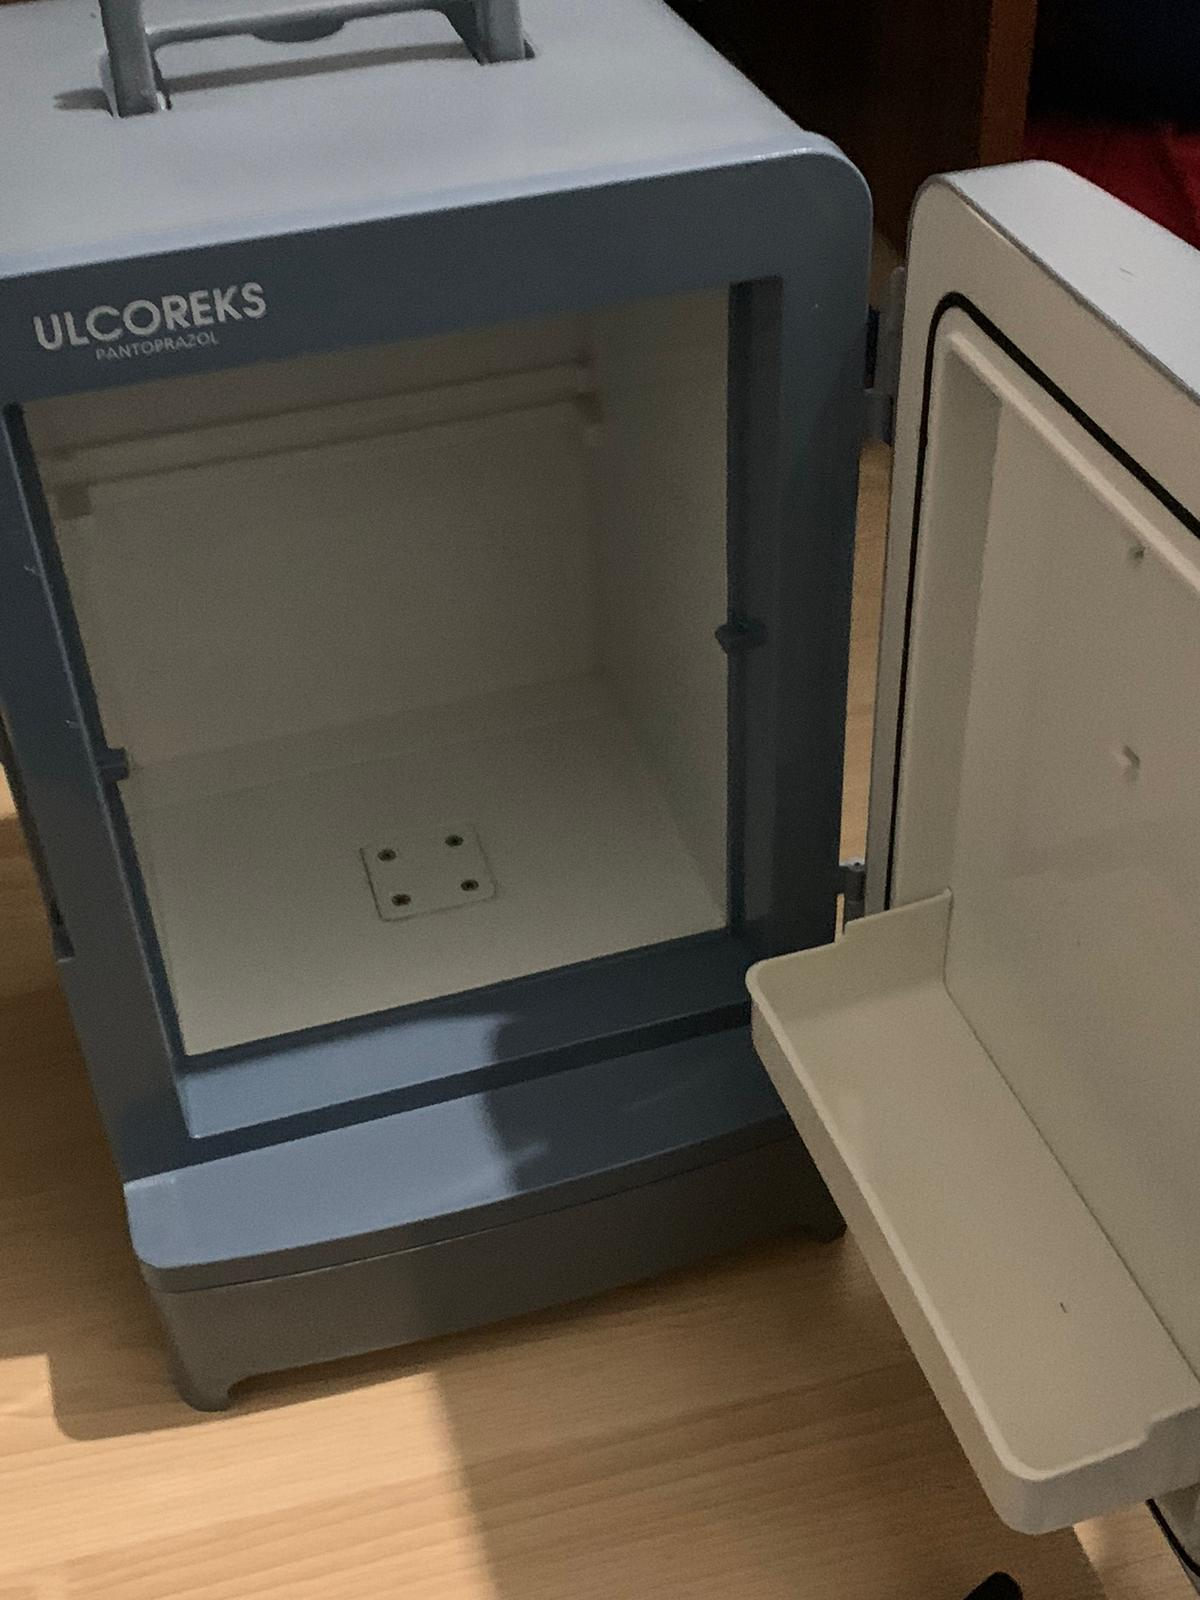
\includegraphics[width=1\textwidth]{Imgs/minibar.jpg}
    \caption{\label{fig:pic1}Minibar.}
\end{figure}

\begin{figure}[!htbp]
    \centering
    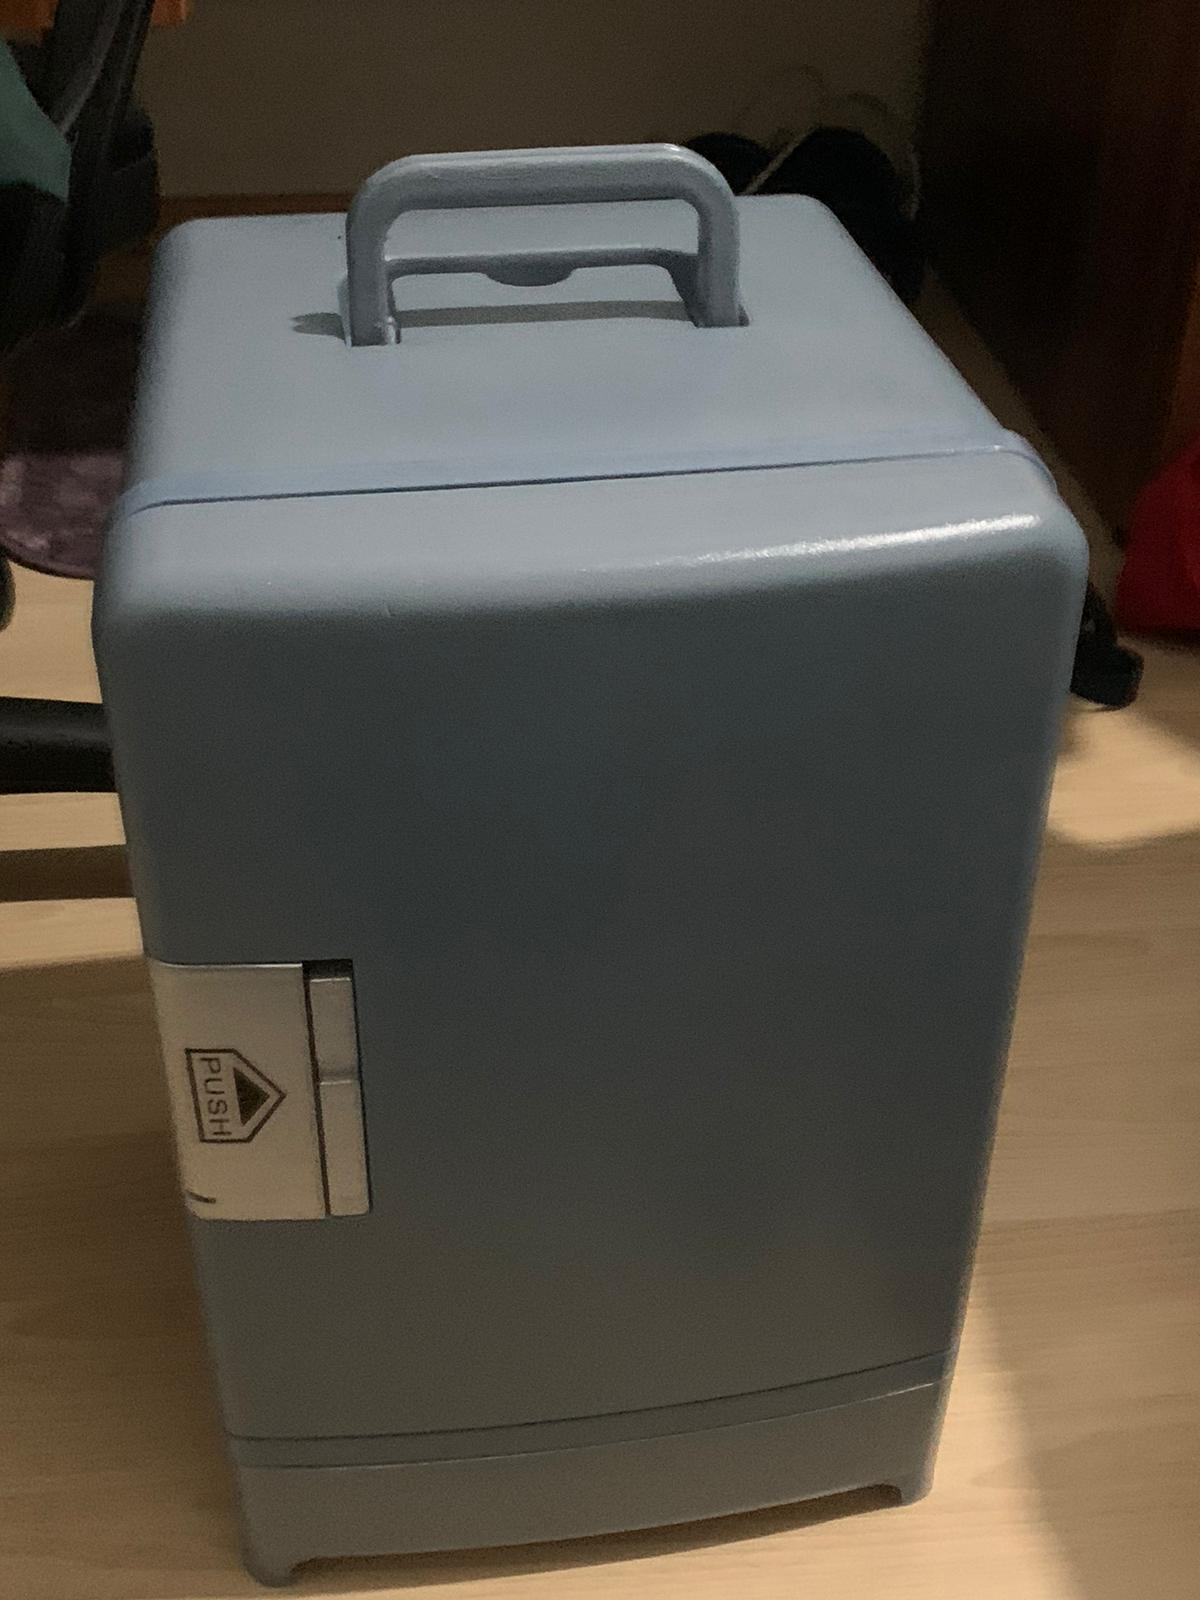
\includegraphics[width=1\textwidth]{Imgs/minibar2.jpg}
    \caption{\label{fig:pic1}Minibar.}
\end{figure}

\chapter{Literature Review}
In my literature review, I focused on exploring the advancements in object detection models, specifically MobileNet SSD v2. I examined academic papers that documented the evolution of the MobileNet SSD architecture and its application in real-time object detection tasks. By studying these papers, I gained insights into the key features, innovations, and performance improvements introduced in different versions of MobileNet SSD, such as MobileNet SSD v2.

\section{Object Detection: Literature Review}
This section provides a chronological review of key works in the field of object detection, with a focus on the MobileNet SSD v2 model

\subsection{MobileNet: "MobileNets: Efficient Convolutional Neural Networks for Mobile Vision Applications" (Andrew G. Howard et al., arXiv 2017}
This seminal work introduced the MobileNet architecture, which aimed to provide efficient and lightweight convolutional neural networks for mobile devices. MobileNet's depth-wise separable convolutions significantly reduced the computational cost while maintaining reasonable accuracy for object detection tasks.

\subsection{SSD: "SSD: Single Shot MultiBox Detector" (Wei Liu et al., ECCV 2016)}
The SSD model proposed a single-shot approach for object detection, eliminating the need for region proposal networks. It used a series of convolutional layers with different scales to detect objects at multiple resolutions, improving speed and accuracy.

\subsection{MobileNet SSD: "MobileNetV2: Inverted Residuals and Linear Bottlenecks" (Mark Sandler et al., CVPR 2018)}
Building upon the MobileNet architecture, MobileNet SSD introduced additional modifications to enable object detection capabilities. It incorporated the SSD framework into MobileNet, achieving real-time object detection on mobile and embedded devices.

\subsection{MobileNet SSD v2: "MobileNetV2: The Next Generation of On-Device Computer Vision Networks" (Mark Sandler et al., CVPR 2018)}
MobileNet SSD v2 further improved the MobileNet architecture with novel design choices. It introduced inverted residuals, linear bottlenecks, and improved feature extraction capabilities. These enhancements resulted in increased accuracy and efficiency compared to the previous versions.

\subsection{EfficientDet: "Scalable and Efficient Object Detection" Mingxing Tan et al., CVPR 2020}
While not directly related to MobileNet SSD v2, EfficientDet presented a scalable and efficient object detection architecture. It introduced a compound scaling method that achieved state-of-the-art performance by balancing model size, computational cost, and accuracy. EfficientDet can serve as a complementary reference for optimizing object detection models.

\subsection{Mask R-CNN (Kaiming He et al., ICCV 2017)}
An extension of Faster R-CNN that not only detects objects, but also the full shape (mask) of objects. This proved to be very effective in image segmentation tasks.

\subsection{Cascade R-CNN: ”Delving into High Quality Object Detection” (Zhaowei Cai and Nuno Vasconcelos, CVPR 2018)}
Proposed a cascaded R-CNN configuration to improve detection quality, increasing the accuracy of bounding boxes

\subsection{Why MobileNet SSD v2?}
\begin{itemize}
    \item MobileNet Architecture: MobileNet SSD v2 is built upon the MobileNet architecture, which is designed to provide efficient and lightweight convolutional neural networks for mobile and embedded devices. It utilizes depth-wise separable convolutions to reduce computational complexity while maintaining reasonable accuracy.
    \item Inverted Residuals: MobileNet SSD v2 introduces the concept of inverted residuals, which aim to improve the flow of information through the network. Inverted residuals use a bottleneck layer with a linear projection followed by non-linear transformations, enabling more efficient feature extraction.
    \item Linear Bottlenecks: The linear bottlenecks in MobileNet SSD v2 help to reduce the number of parameters and computational cost. By applying a linear activation function to bottleneck layers, the network achieves better utilization of model capacity and improves performance.
    \item Feature Pyramid Network (FPN): MobileNet SSD v2 incorporates a feature pyramid network, which allows the model to capture multi-scale features from different layers of the network. This helps in detecting objects of various sizes and improves the accuracy of object detection.
    \item SSD Framework: MobileNet SSD v2 follows the Single Shot MultiBox Detector (SSD) framework, which eliminates the need for region proposal networks and enables real-time object detection. It uses a set of convolutional layers with different scales to detect objects at multiple resolutions, facilitating accurate and efficient detection.
\end{itemize}

\chapter{Dataset}

Object detection in minibars involves the use of computer vision techniques and object detection models to identify and track items inside the minibar. In this project, I trained photos that captured in minibar for getting better results in minibar.


\section{Processing Dataset}

\subsection{Objective}
Take pictures from minibar with webcam and label them for processing.Divide parts images for 80 percent train,
10 percent validation, 10 percent test.

\subsection{Libraries and Modules Used}
The process uses Python libraries and modules including pandas, numpy,os and some scripts. These libraries provide necessary functions for data processing.

\subsection{Scripts}
Scripts are mainly used for dividing pictures for train,test,validation; create labelmap txt for classes; create model, convert model tensorflow lite etc.

\subsection{Data Download and Processing}
Bounding boxes are created by label img. They are then filtered according to the classes specified by the user. 

In summary, user took images from minibar with different angles and all objects on the scene. Then labels all images with any label program for preparing training.

\subsection{Tensorflow Setup}
Tensorflow is required for using webcam or raspi cam with object recognition projects.For installing tensorflow we can follow this steps:

\subsection{Controlling version, then Installing Tensorflow and Python}
Start by setting up our Raspberry Pi with the latest version of Raspberry Pi OS with sudo apt update command.
Then install the required dependencies by running the sudo apt install libatlas-base-dev command.Then install python package with sudo apt install python3-pip and finally pip3 install tensorflow.

\subsection{Images From The Dataset}

\begin{figure}[!htbp]
    \centering
    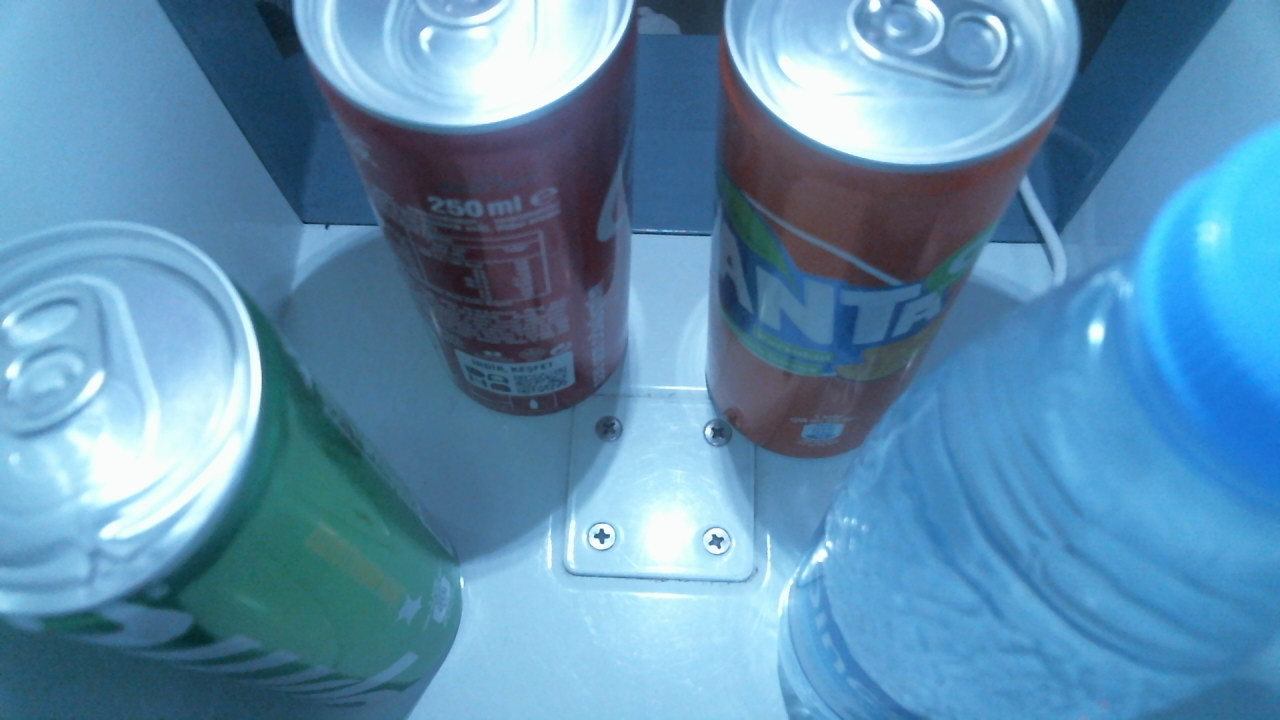
\includegraphics[width=1\textwidth]{Imgs/datasetphotos1.jpg}
    \caption{\label{fig:pic1}Photos from dataset.}
\end{figure}
\begin{figure}[!htbp]
    \centering
    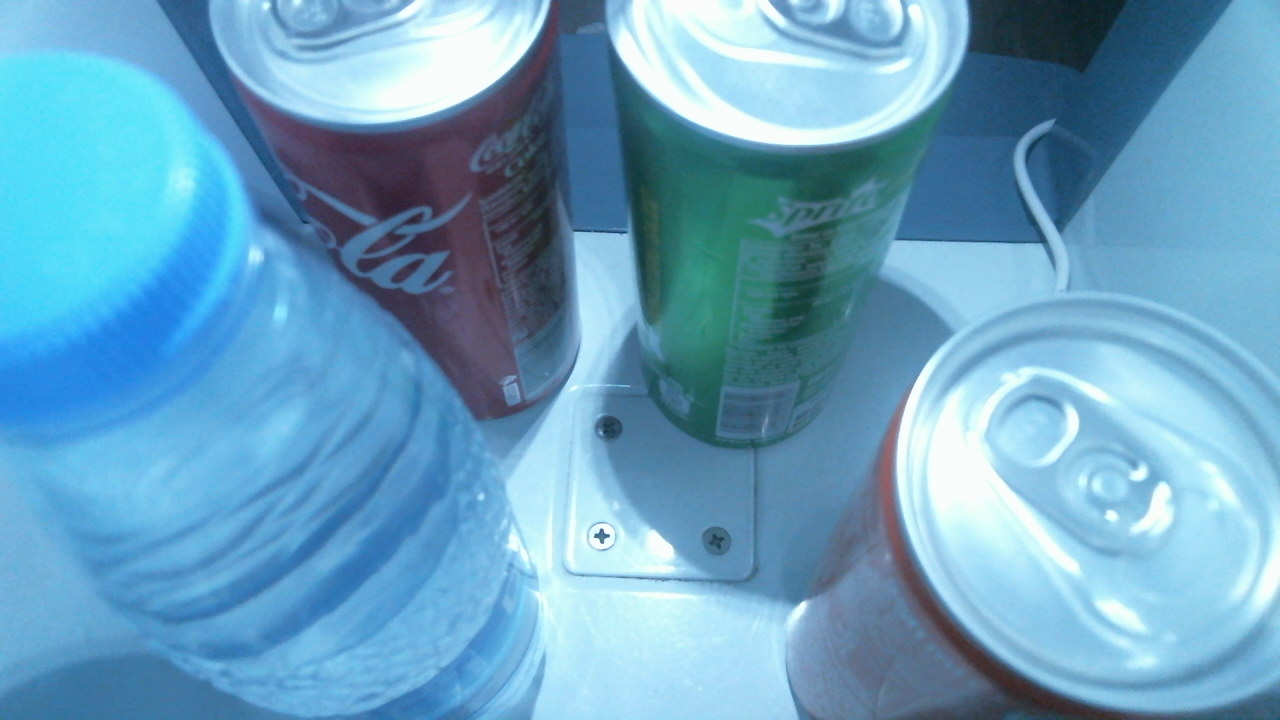
\includegraphics[width=1\textwidth]{Imgs/datasetphotos2.jpg}
    \caption{\label{fig:pic2}Photos from dataset.}
\end{figure}
\begin{figure}[!htbp]
    \centering
    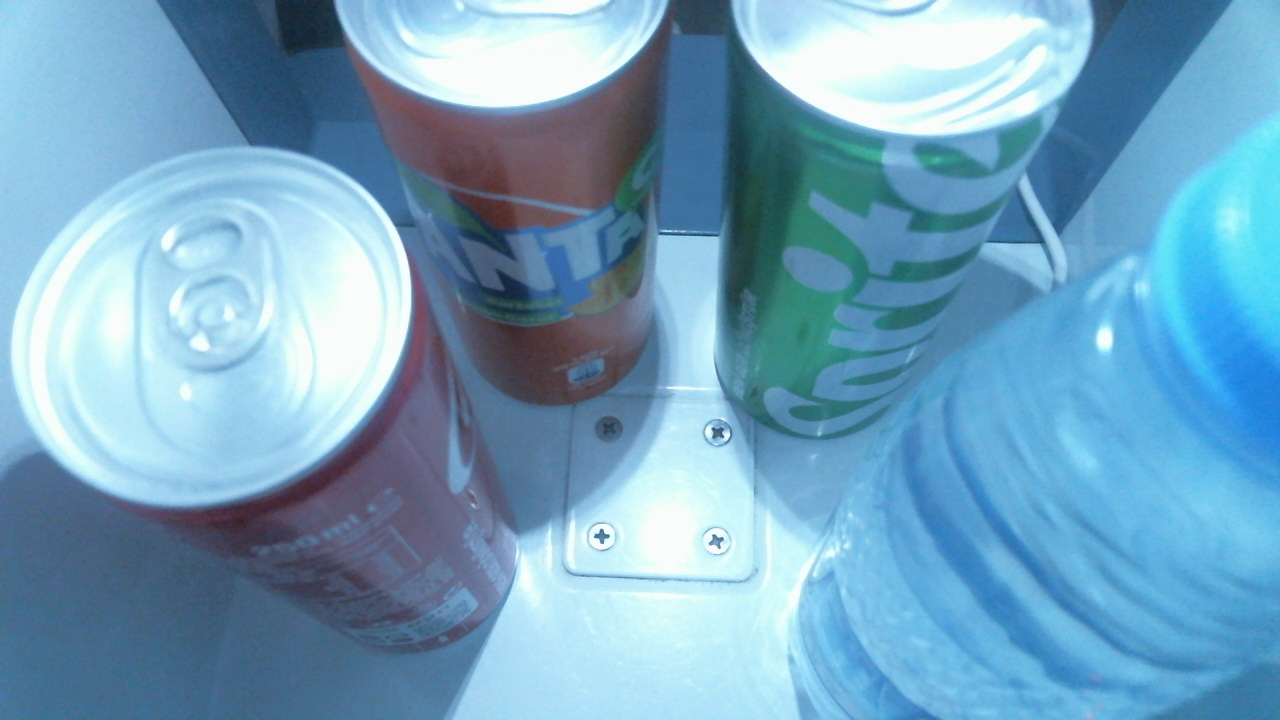
\includegraphics[width=1\textwidth]{Imgs/datasetphotos3.jpg}
    \caption{\label{fig:pic3}Photos from dataset.}
\end{figure}

\subsection{Resources}
Dataset can easily be created and labelled by How to Capture and Label Training Data to Improve Object Detection Model Accuracy namely youtube video.

\chapter{Object Detection using SSD Mobilenet V2}

In this project, I developed a object detection model based on the SSD Mobilenet V2 version with the purpose of detecting four different objects (cola fanta sprite water). The focus was detecting and counting objects in minibar with best accuracy. During the project, different datasets trained for getting best results. The process and results are discussed below. 

\section{Training steps}

The model is trained in 40000 steps and 16 batch size.
\begin{figure}[!htbp]
    \centering
    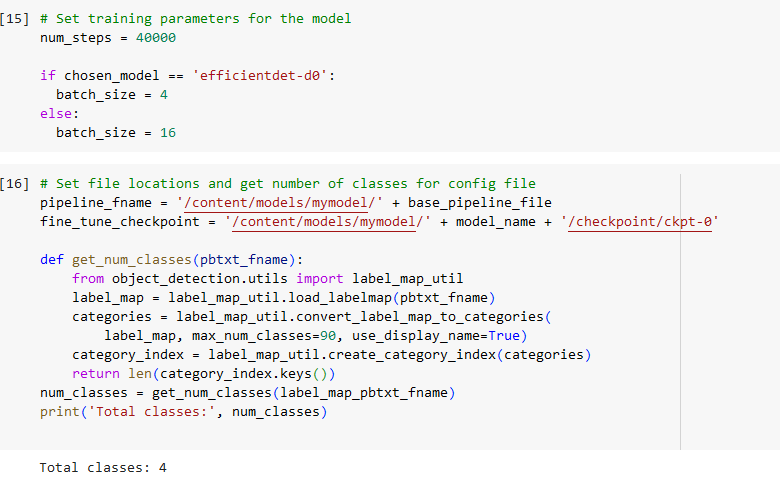
\includegraphics[width=1\textwidth]{Imgs/parameters.PNG}
    \caption{\label{fig:parameters}Parameters }
\end{figure}

\begin{figure}[!htbp]
    \centering
    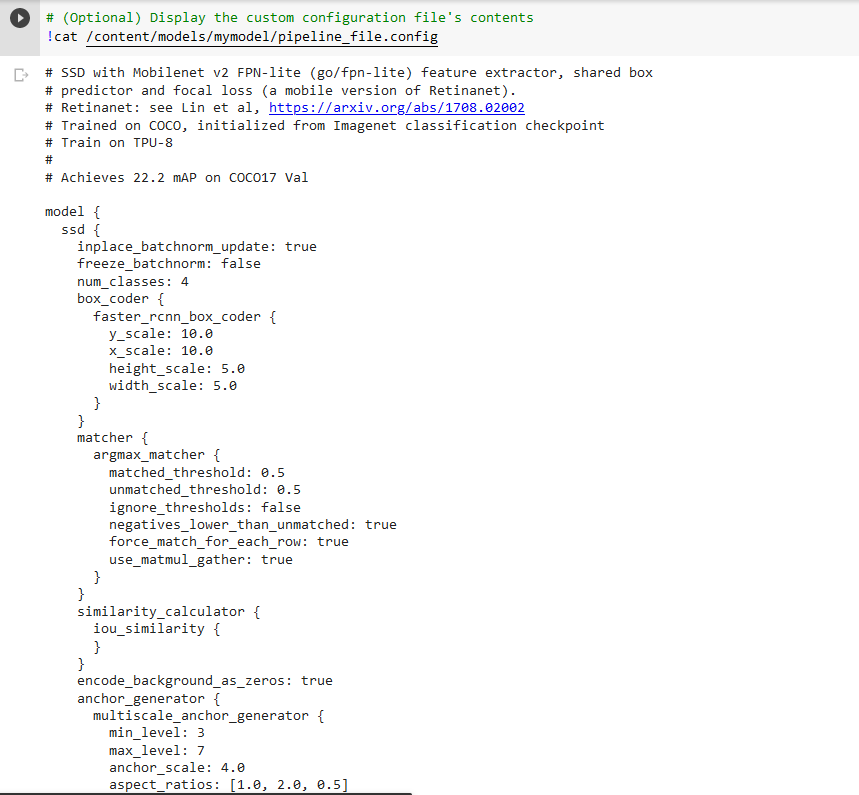
\includegraphics[width=0.6\textwidth]{Imgs/trainconfig.png}
    \caption{\label{fig:train_config}Parameters }
\end{figure}
\begin{figure}[!htbp]
    \centering
    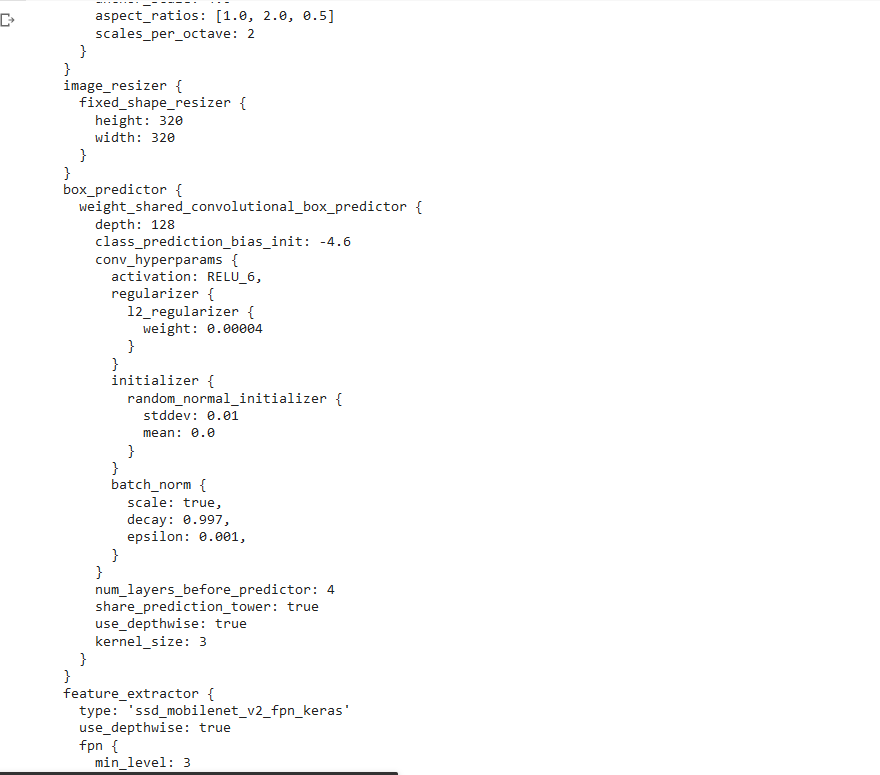
\includegraphics[width=0.6\textwidth]{Imgs/trainconfig2.png}
    \caption{\label{fig:train_config}Parameters }
\end{figure}
\begin{figure}[!htbp]
    \centering
    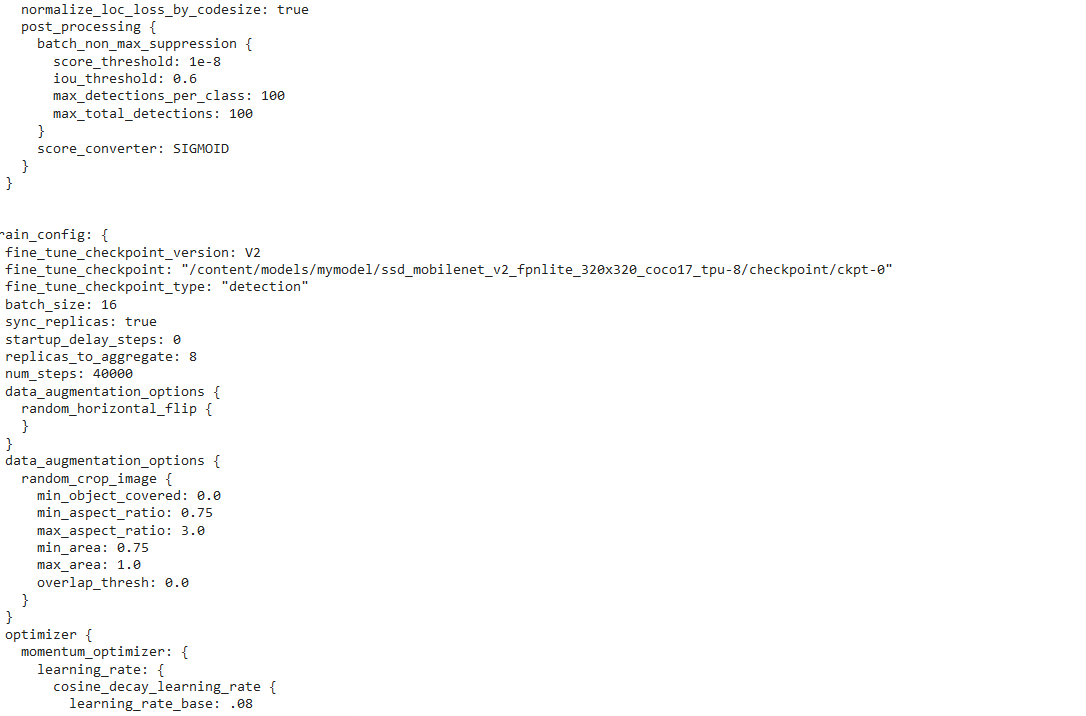
\includegraphics[width=0.6\textwidth]{Imgs/training_parameters.png}
    \caption{\label{fig:train_params}Parameters }
\end{figure}

\subsection{Training Results}
Threshold results of training:
\begin{figure}[!htbp]
    \centering
    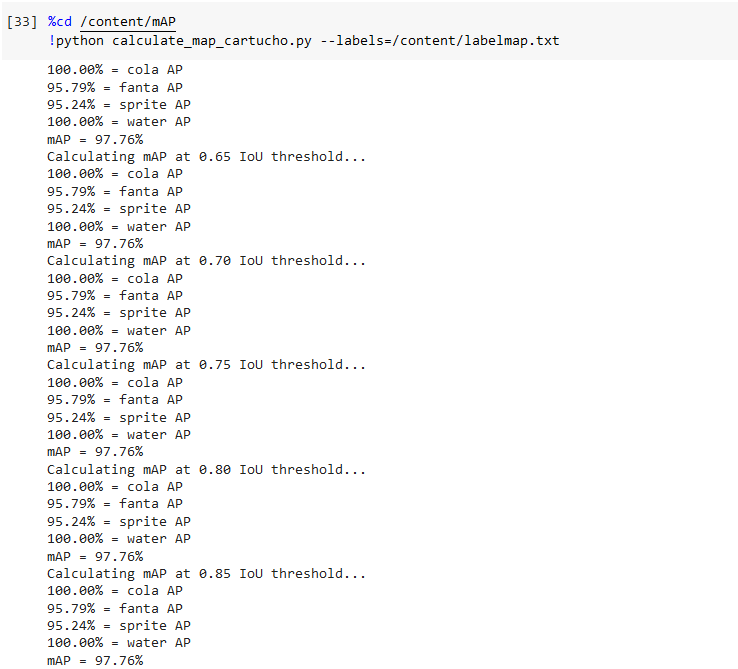
\includegraphics[width=0.6\textwidth]{Imgs/threshold1.PNG}
    \caption{\label{fig:threshold}Threshold }
\end{figure}
\begin{figure}[!htbp]
    \centering
    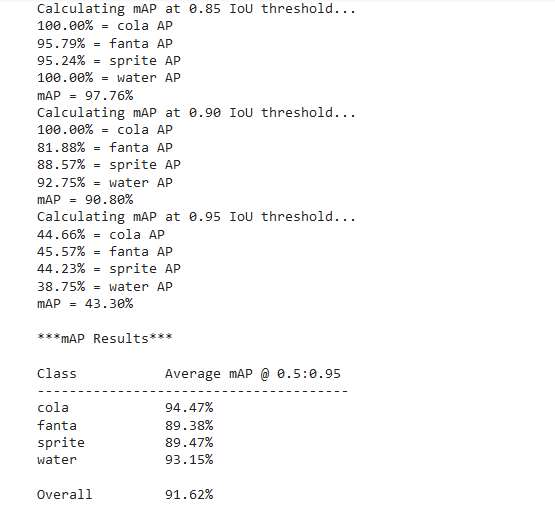
\includegraphics[width=0.6\textwidth]{Imgs/threshold2.PNG}
    \caption{\label{fig:threshold}Threshold }
\end{figure}

\subsection{Learning rate and loss of model}
Here is the rate of model learning. We can see that learning rate schedules in deep learning models often involve an initial phase where the learning rate is relatively high, followed by a gradual decrease over time. This pattern of a learning rate that "peaks" before decreasing serves several purposes.

\begin{figure}[!htbp]
    \centering
    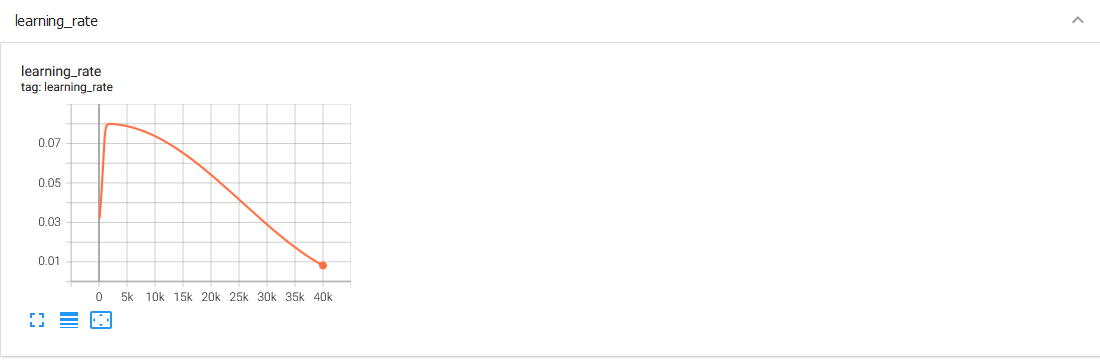
\includegraphics[width=0.8\textwidth]{Imgs/learning_rate.png}
    \caption{\label{fig:learning_rate}Learning rate}
\end{figure}
\\

Loss is s a measure of how well a model's predictions align with the true values or labels of the training data. The loss quantifies the error or mismatch between the predicted output of the model and the desired output.

During the training process, the model iteratively adjusts its parameters or weights to minimize the loss. By minimizing the loss, the model aims to improve its ability to make accurate predictions on unseen data.

\begin{figure}[!htbp]
    \centering
    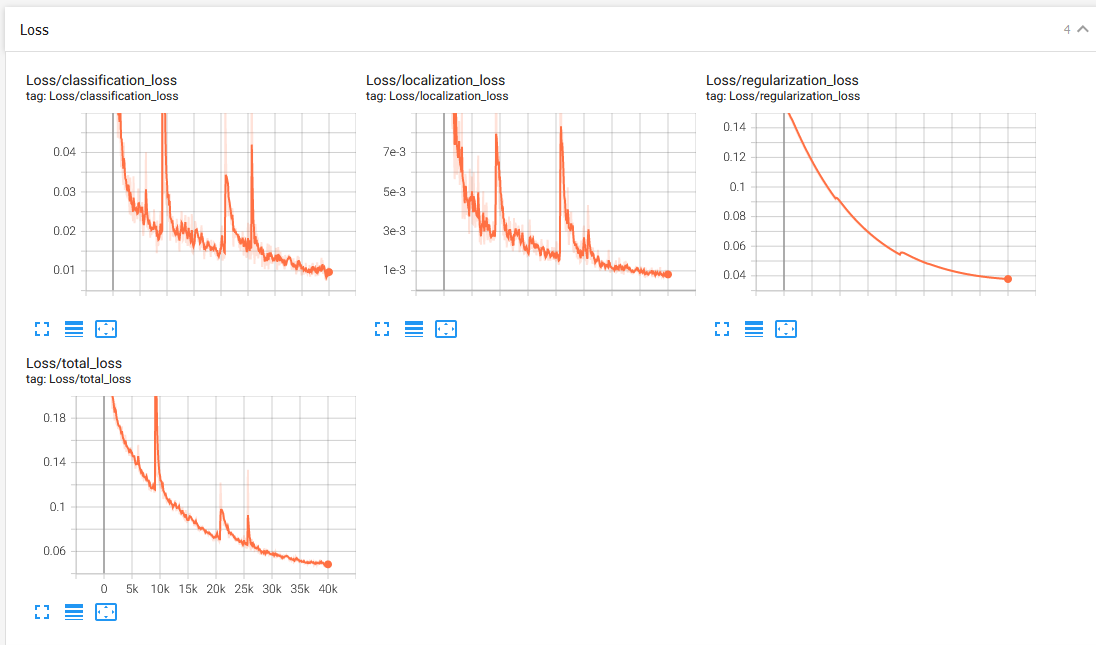
\includegraphics[width=0.9\textwidth]{Imgs/loss.PNG}
    \caption{\label{fig:loss}Loss}
\end{figure}

Detecting and counting four object:

\begin{figure}[!htbp]
    \centering
    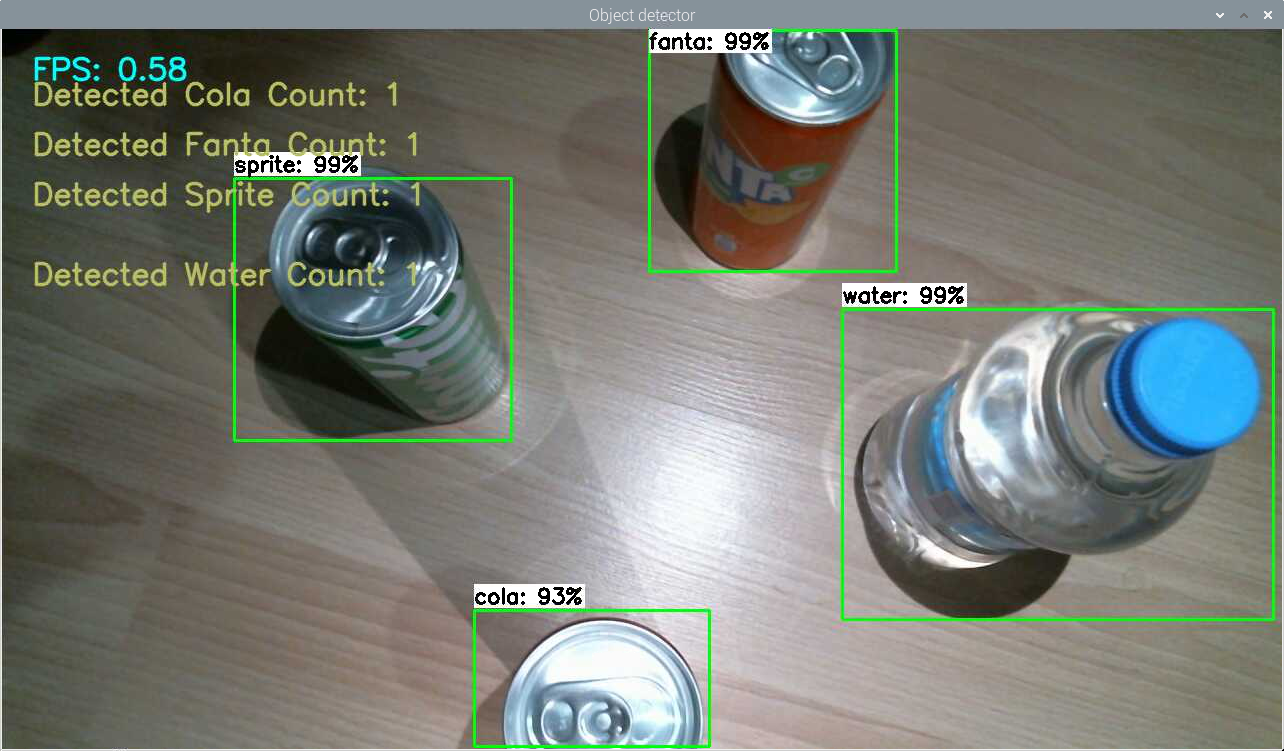
\includegraphics[width=0.9\textwidth]{Imgs/object_counts.PNG}
    \caption{\label{fig:loss}Object Detection and Counts}
\end{figure}


\chapter{Connecting Database}
For real time database I used firabase real time database system.Because Firebase offers easy integration with various platforms and frameworks and Firebase allows us to extend application's functionality with serverless Cloud Functions.

\section{Steps for creating real time database in Firebase}
Navigate to the Realtime Database section of the Firebase console.And select create new database.Then I needed to install raspbbery some libraries for communicating with database

\subsection{Install to raspberry}
Firstly install pyrabase with this command pip install pyrebase. Then get required informations and fill this parts config\\
    "apiKey"\\
    "authDomain"\\
    "databaseURL"\\
    "storageBucket"\\

With this informations raspi easily interact with firebase. For getting key we need to create add an user to authentication then we get api key and connect easily.

\subsection{Usage}
With adding required codes to main program, we add customers and products to our database.And send count of products to database. If count of product in minibar is reduced in a time(user take a product from minibar), raspberry detects that and decrease count of product and updates customers bill.
\begin{figure}[!htbp]
    \centering
    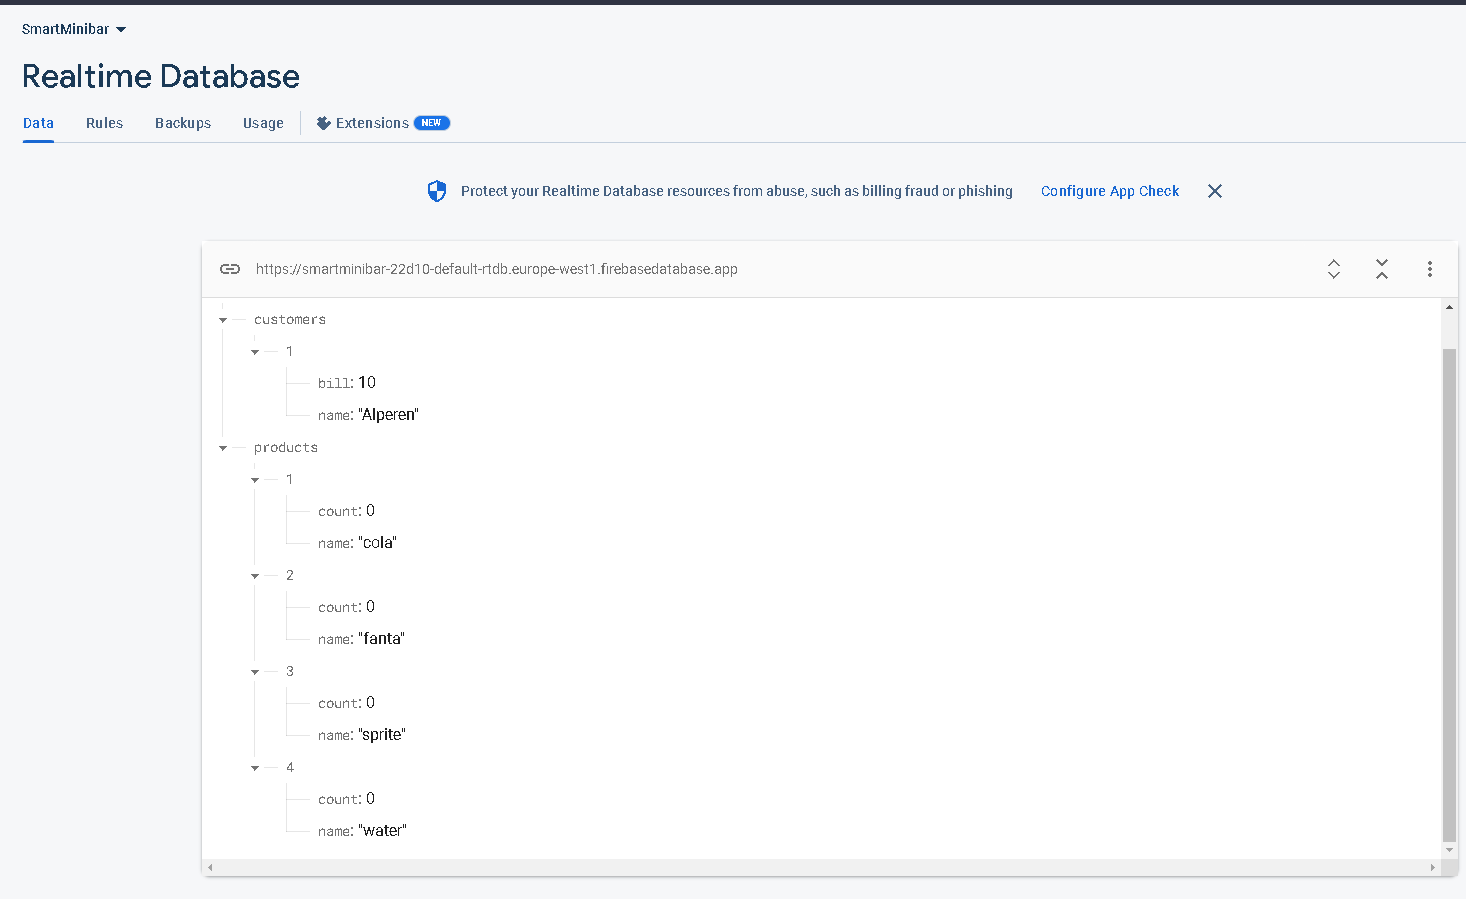
\includegraphics[width=0.8\textwidth]{Imgs/databasefirebase.png}
    \caption{\label{fig:Firabase}Firabase connection.}
\end{figure}
\\

\begin{figure}[!htbp]
    \centering
    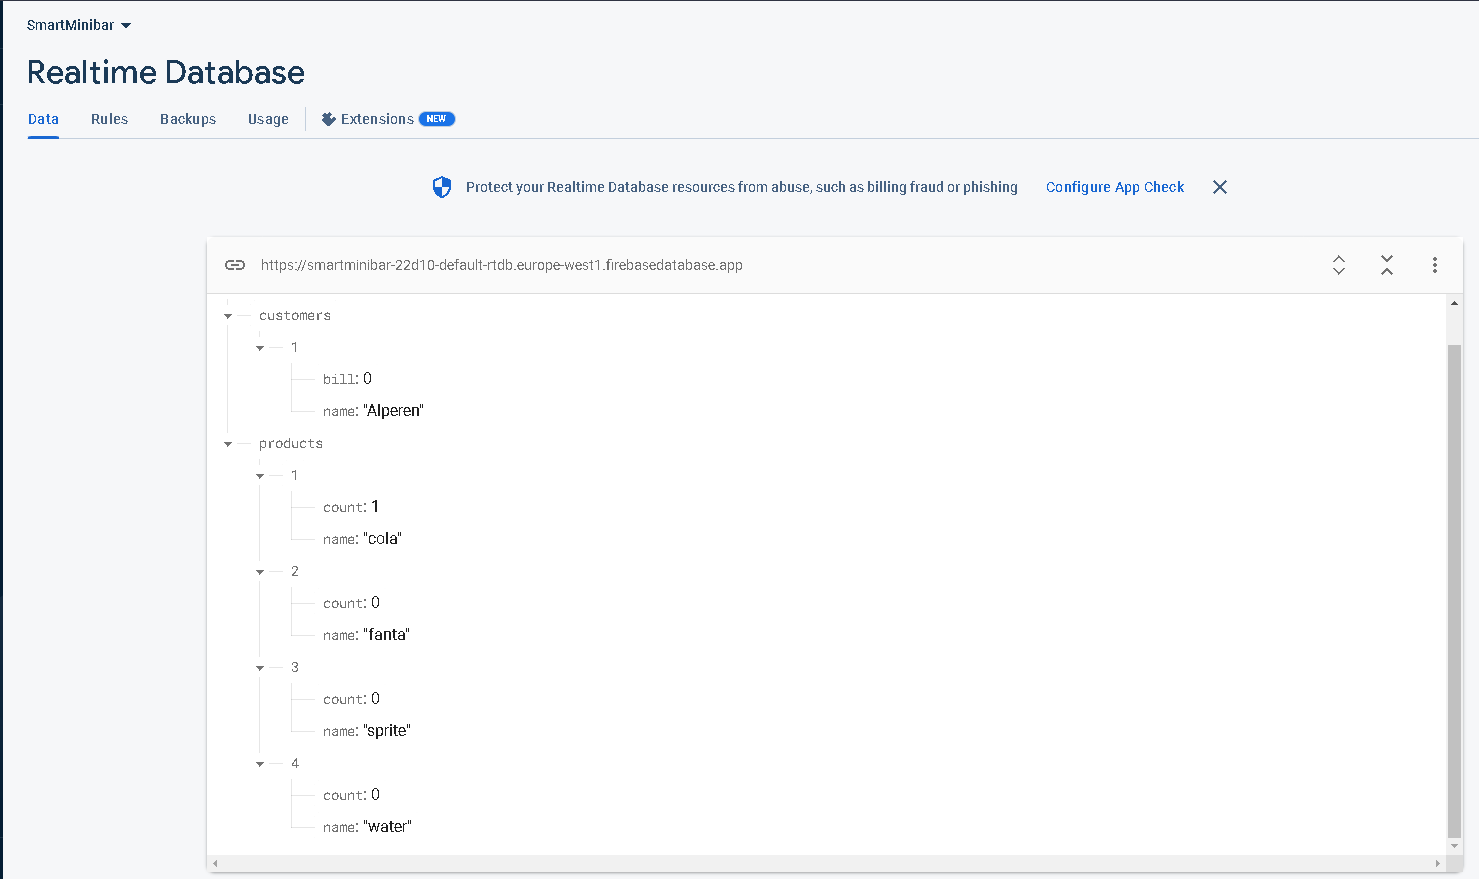
\includegraphics[width=0.8\textwidth]{Imgs/firebase1.png}
    \caption{\label{fig:Firabase}Firabase connection.}
\end{figure}
\\

This photos show when user takes 1 cola from minibar, what happens.
\chapter{Final Steps}

\section{Inserting Items Minibar}

\begin{figure}[!htbp]
    \centering
    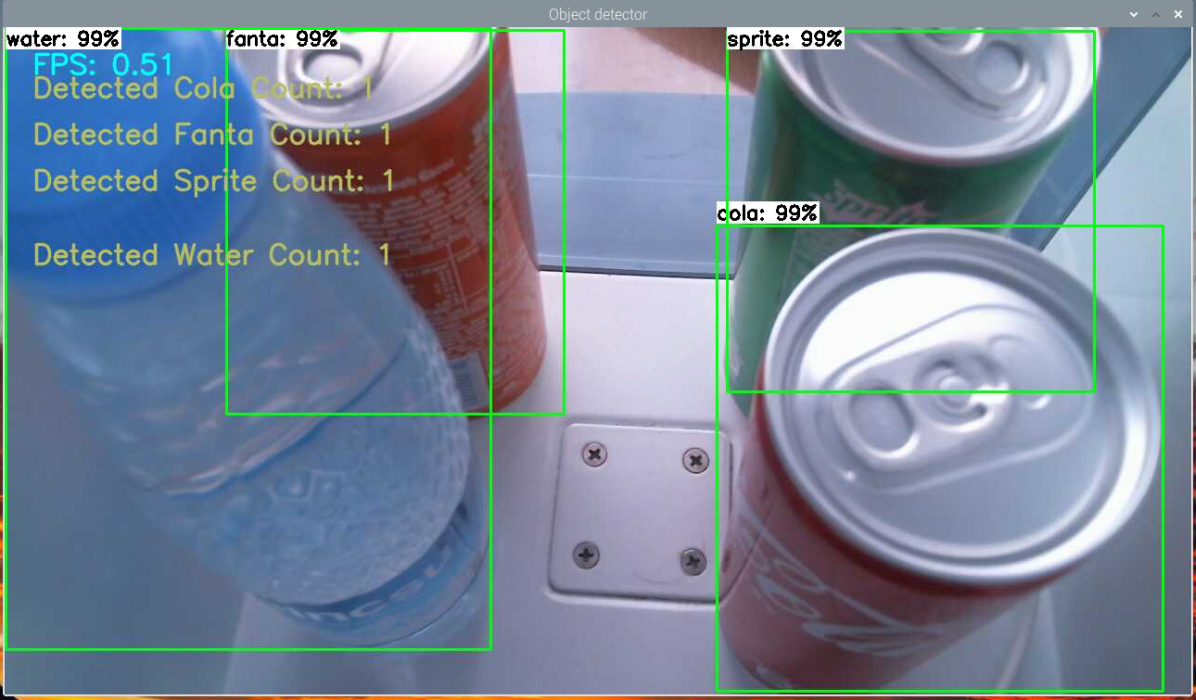
\includegraphics[width=0.9\textwidth]{Imgs/rapor1.PNG}
    \caption{\label{fig:minibar}Photos from minibar}
\end{figure}

\begin{figure}[!htbp]
    \centering
    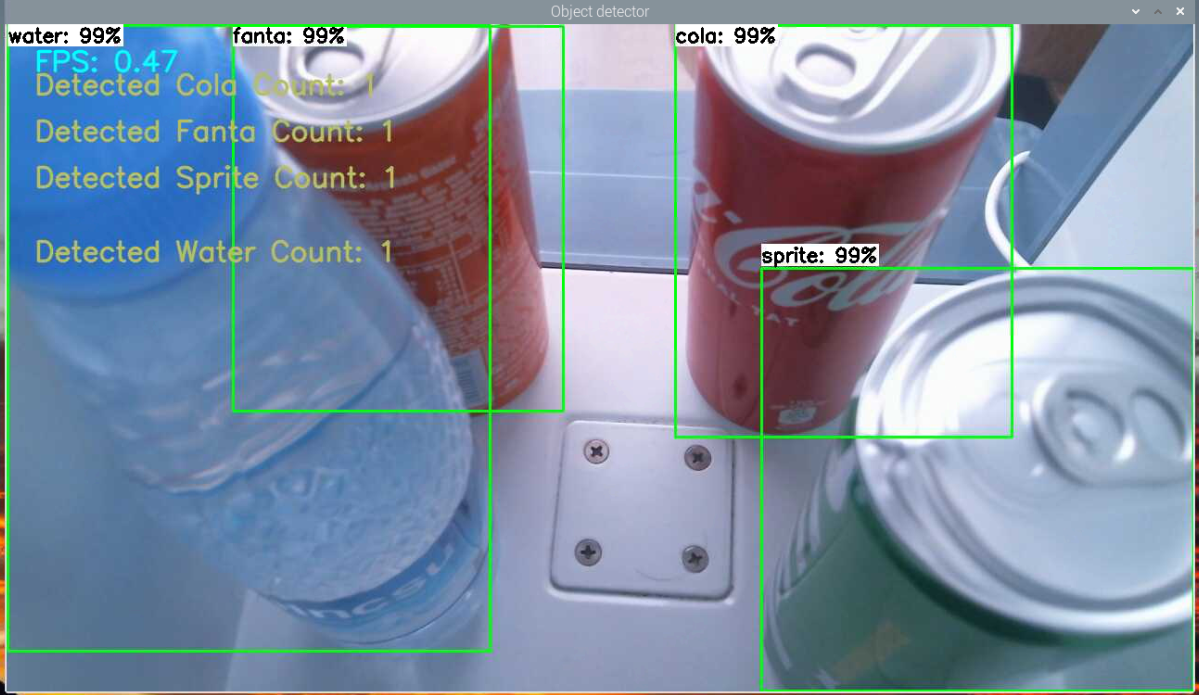
\includegraphics[width=0.9\textwidth]{Imgs/rapor2.PNG}
    \caption{\label{fig:minibar}Photos from minibar}
\end{figure}

\begin{figure}[!htbp]
    \centering
    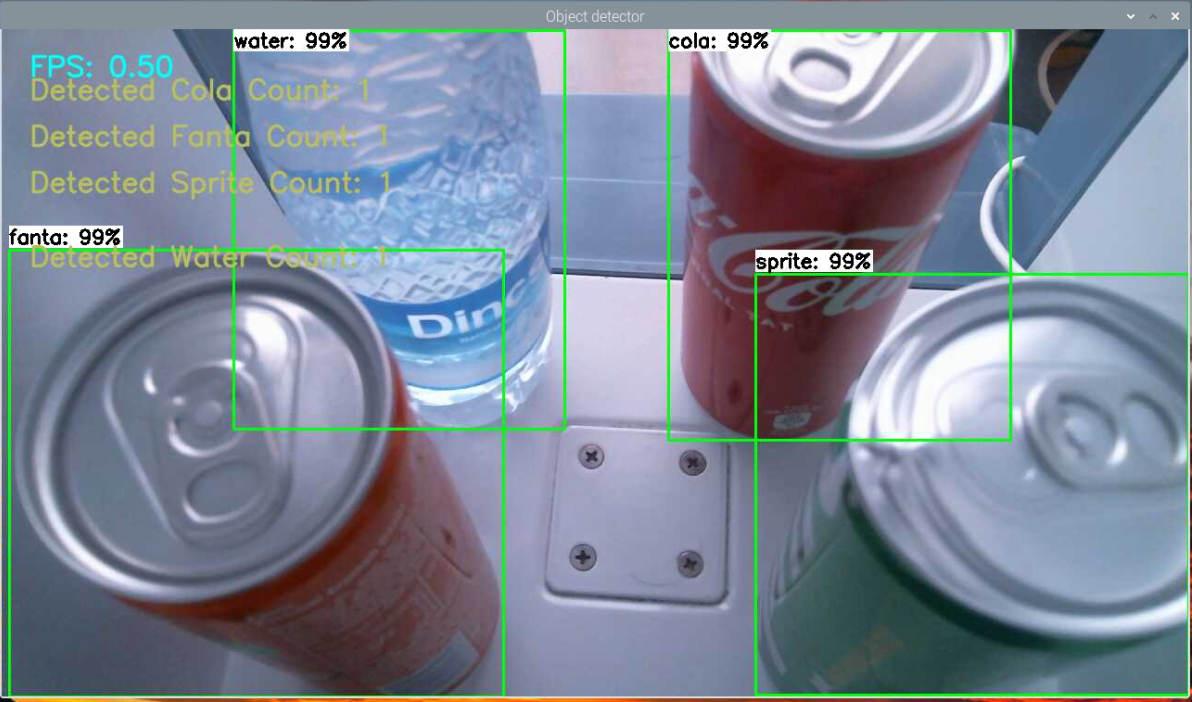
\includegraphics[width=0.9\textwidth]{Imgs/rapor3.PNG}
    \caption{\label{fig:minibar}Photos from minibar}
\end{figure}

\begin{figure}[!htbp]
    \centering
    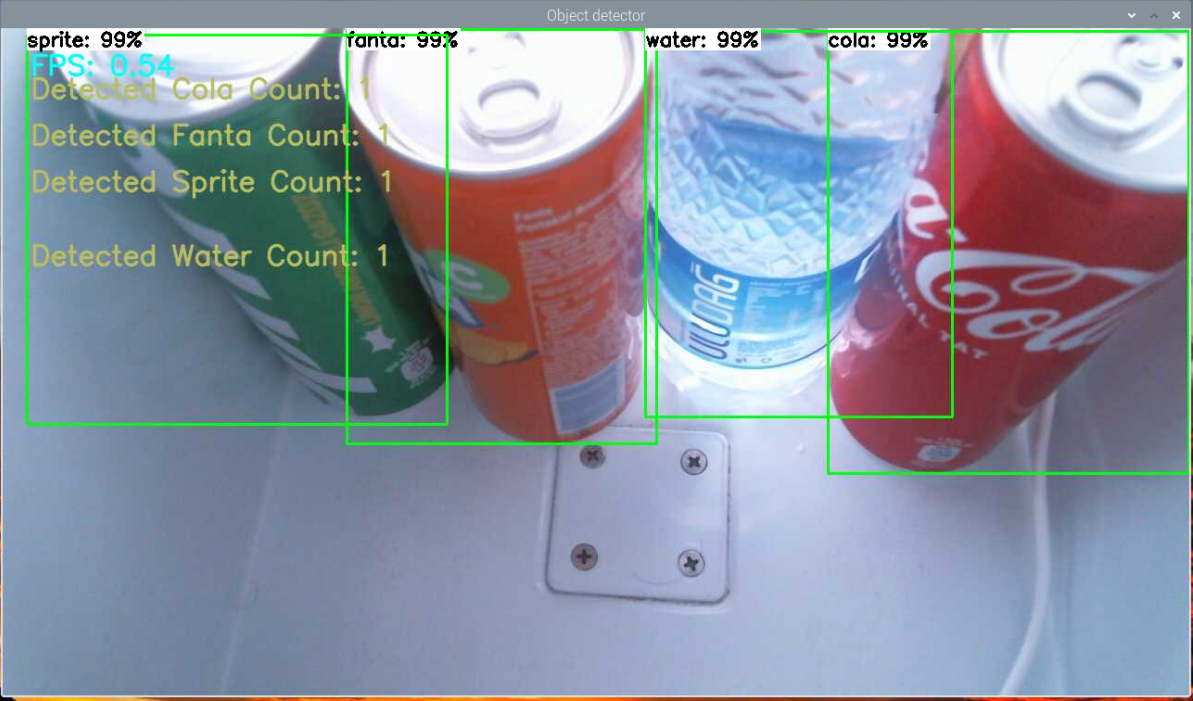
\includegraphics[width=0.9\textwidth]{Imgs/rapor4.PNG}
    \caption{\label{fig:minibar}Photos from minibar}
\end{figure}

\subsection{Products inside minibar}
All products inside minibar.
\begin{figure}[!htbp]
    \centering
    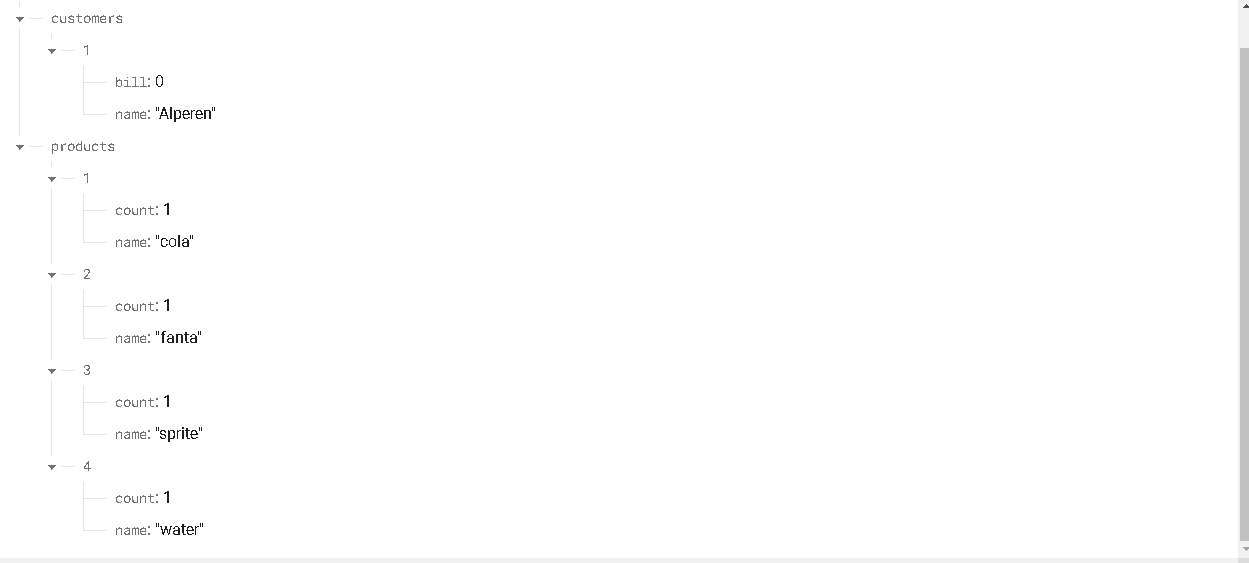
\includegraphics[width=0.9\textwidth]{Imgs/beforetaking cola.PNG}
    \caption{\label{fig:products in minibar}Products from minibar}
\end{figure}

\begin{figure}[!htbp]
    \centering
    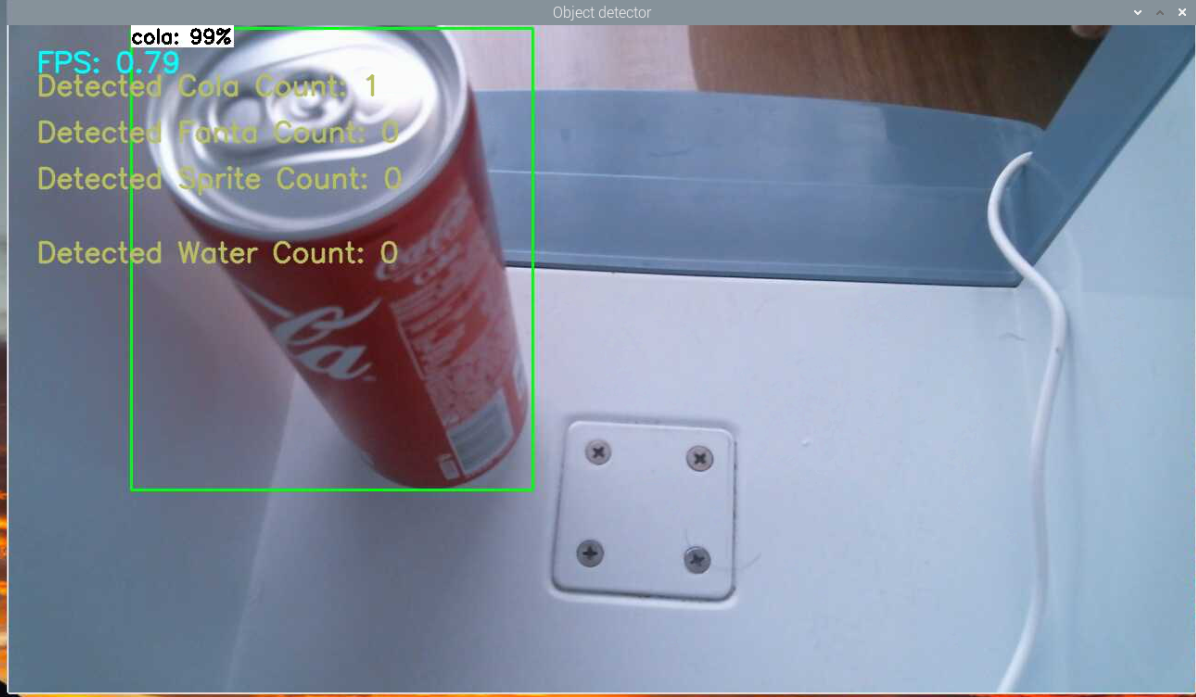
\includegraphics[width=0.9\textwidth]{Imgs/only cola.PNG}
    \caption{\label{fig:products in minibar}Products from minibar}
\end{figure}

\begin{figure}[!htbp]
    \centering
    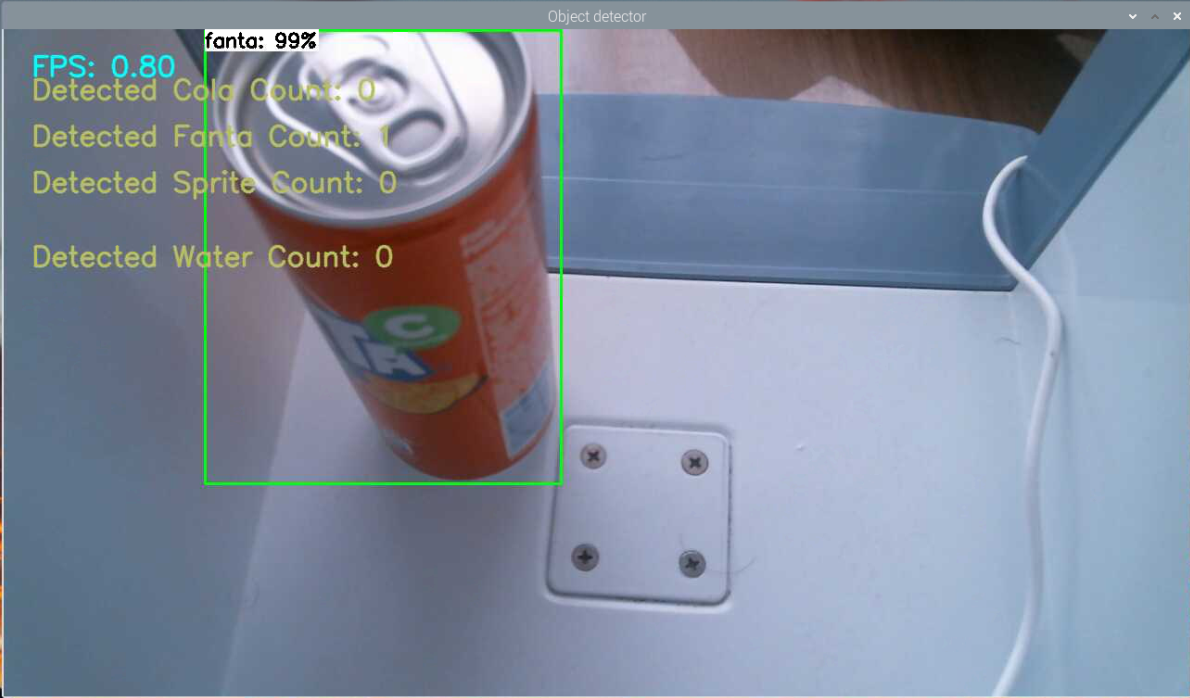
\includegraphics[width=0.9\textwidth]{Imgs/only fanta.PNG}
    \caption{\label{fig:products in minibar}Products from minibar}
\end{figure}

\begin{figure}[!htbp]
    \centering
    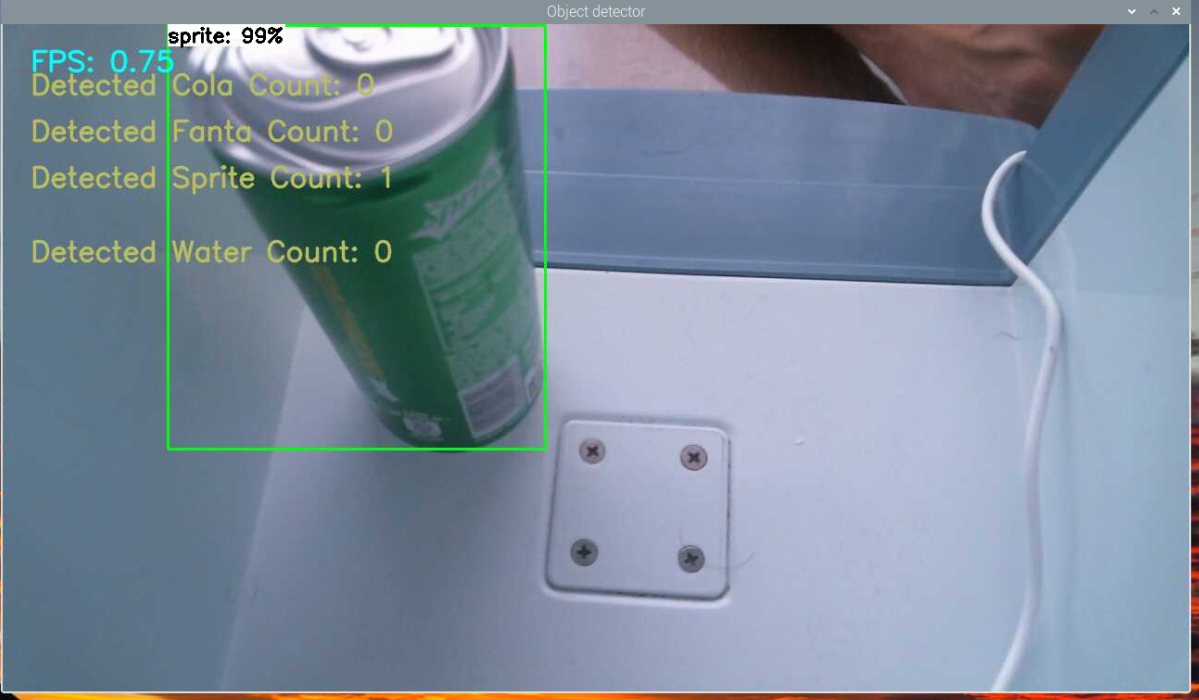
\includegraphics[width=0.9\textwidth]{Imgs/only sprite.PNG}
    \caption{\label{fig:products in minibar}Products from minibar}
\end{figure}

\begin{figure}[!htbp]
    \centering
    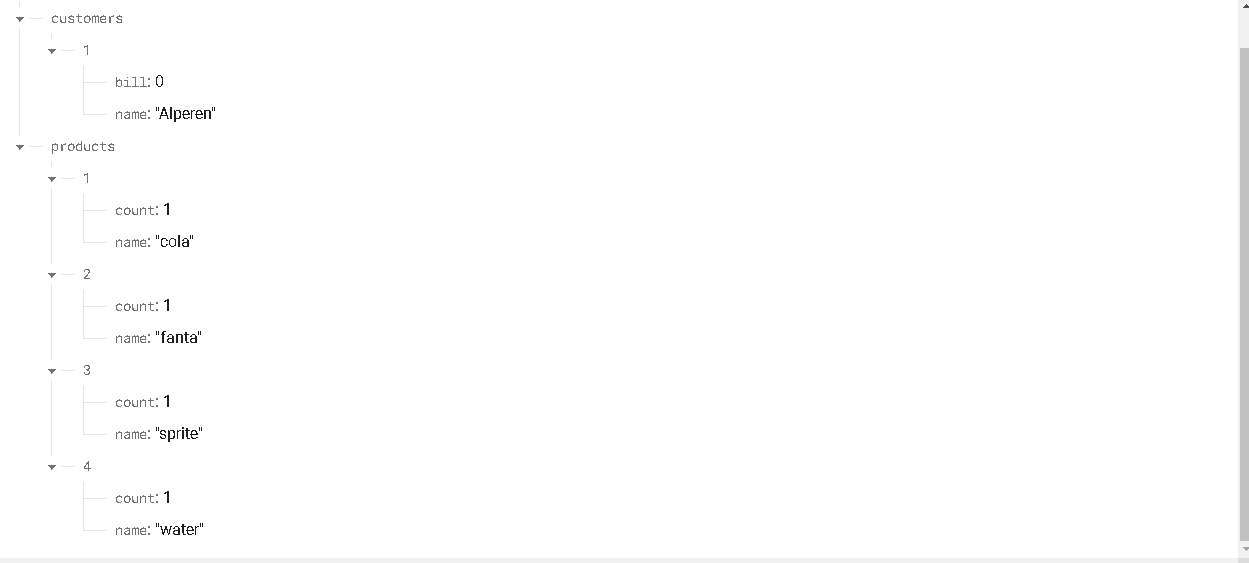
\includegraphics[width=0.9\textwidth]{Imgs/beforetaking cola.PNG}
    \caption{\label{fig:roducts in minibar}Products from minibar}
\end{figure}

\subsection{Taking fanta from minibar}
We are taking fanta and database getting updated. Fanta is 9 cost.
\begin{figure}[!htbp]
    \centering
    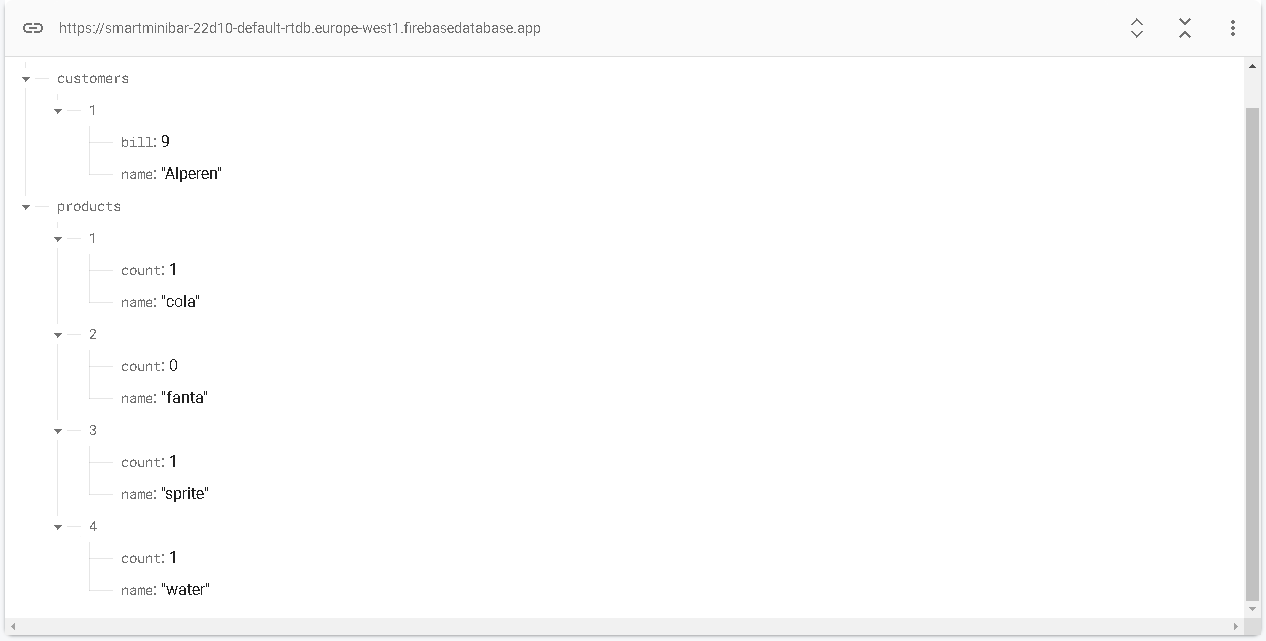
\includegraphics[width=0.9\textwidth]{Imgs/taking fanta.PNG}
    \caption{\label{fig:taking products from minibar}Taking fanta from minibar}
\end{figure}

\subsection{Taking sprite from minibar}
We are taking sprite and database getting updated. Sprite is 8 cost.
\begin{figure}[!htbp]
    \centering
    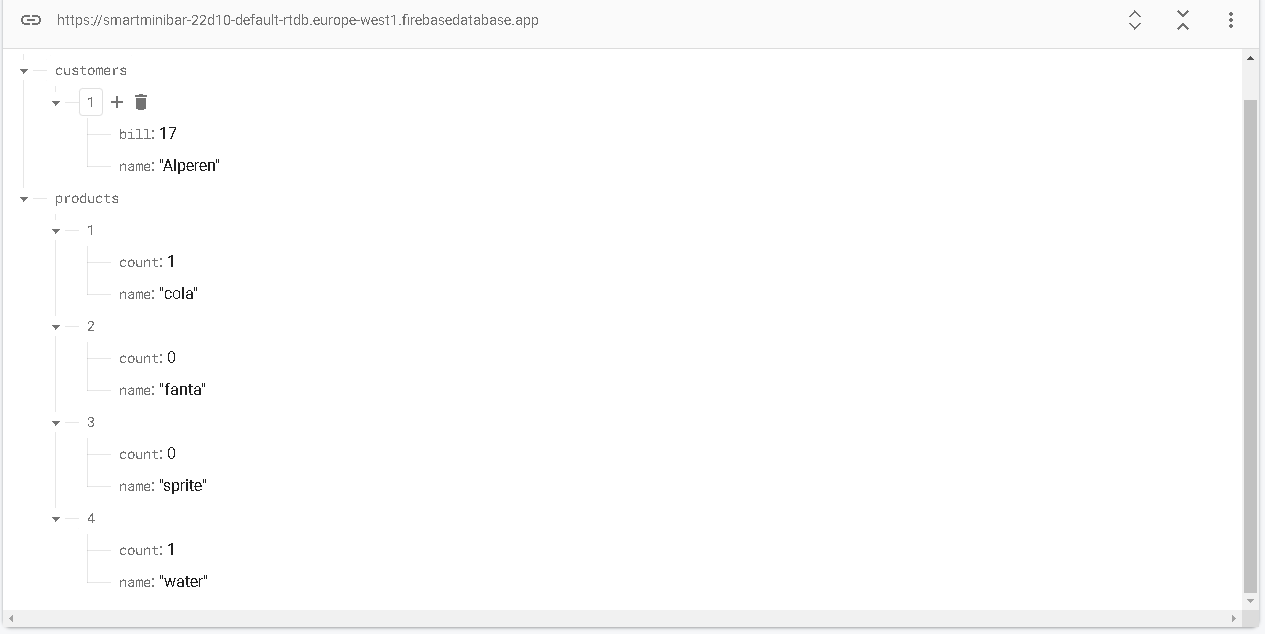
\includegraphics[width=0.9\textwidth]{Imgs/taking sprite.PNG}
    \caption{\label{fig:taking products from minibar}Taking sprite from minibar}
\end{figure}

\subsection{Taking cola and water from minibar}
We are taking both water and cola and database getting updated. Cola is 10 cost and water 7 cost.
\begin{figure}[!htbp]
    \centering
    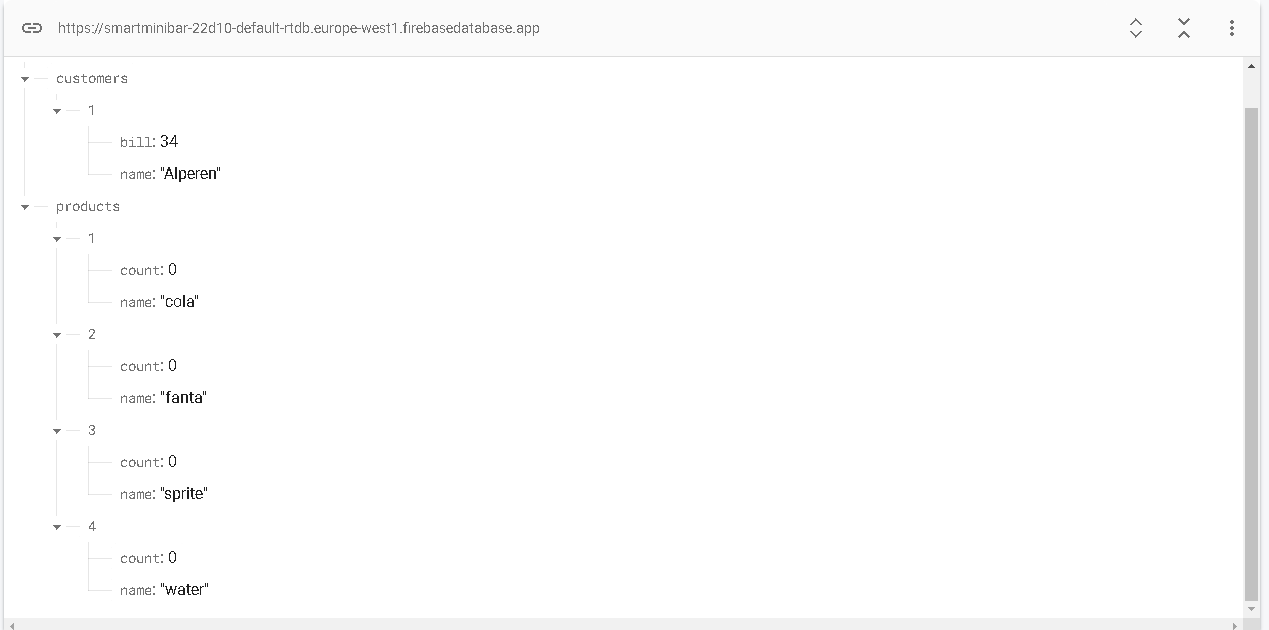
\includegraphics[width=0.9\textwidth]{Imgs/taking cola and water in same time.PNG}
    \caption{\label{fig:taking products from minibar}Taking water from minibar}
\end{figure}







% DON'T INPUT FILES AFTER HERE
\begin{outertitles}
\clearpage
\setlength{\emergencystretch}{1em}
\printbibliography
\addtocontents{toc}{\protect\vspace{18pt}}
\addcontentsline{toc}{chapter}{Bibliography}
%% If you don't want a CV or appendices add a % at the beginning of the relevant line
\chapter*{CV}
\addcontentsline{toc}{chapter}{CV}


\clearpage
|
\end{outertitles}
\end{document}